\documentclass[a4paper,openany,12pt]{book}
\usepackage[a4paper,left=2cm,right=2cm,top=0.5cm,bottom=0.5cm,includehead,includefoot,headheight=0.1cm,heightrounded]{geometry}
\usepackage{amsmath}
\usepackage{graphics}
\usepackage{graphicx}
\usepackage[table,xcdraw]{xcolor}
\usepackage{float}
\usepackage[pro]{fontawesome5}
\usepackage{ragged2e}
\usepackage{titlesec}
\usepackage{tikz}
\usepackage{trimclip}
\usepackage[printwatermark]{xwatermark}
\usepackage{amssymb}
\usepackage[export]{adjustbox}
\usepackage{tocloft}
\usepackage{etoolbox}
\usepackage{algpseudocode}
\renewcommand{\contentsname}{\normalfont \sffamily \huge \textcolor{id7-aubergine}{Table of Contents}\vspace{-1.25em}}
\renewcommand{\cftsecfont}{\normalfont}
\renewcommand{\cftsecpagefont}{\normalfont}
\usetikzlibrary{automata, positioning, shapes.symbols, arrows, chains, calc}
\usepackage{shellesc}
\usepackage{minted}
\usepackage{syntax}
\usemintedstyle{idseven}
\usepackage{listings}
\usepackage[hidelinks]{hyperref}
%\usepackage[osfigures]{opensans}
\usepackage{lastpage}
\usepackage{fancyhdr}
\usepackage{mdframed}
\usepackage{outlines}
\usepackage{bm}
\usepackage{array}
\usepackage{enumitem}
\usepackage[round]{natbib}
\usepackage{environ}
\usepackage{varwidth}
\usepackage{mathtools}
\usepackage{pagecolor}
\usepackage{wrapfig}
\usepackage{nameref}
\usepackage{fontspec}
\setsansfont{Proxima Nova}
\setmonofont{Ubuntu Mono}
\newfontfamily\warwickfont[
Scale=MatchLowercase
%  Path = fonts/
]{Avenir Next}
\makeatletter
\newcommand*{\currentname}{\@currentlabelname}
\makeatother
\usepackage{csquotes}
\usepackage{newfloat}
\usepackage{caption}
\usepackage[super]{nth}
\titleformat{\chapter}[display]
{\normalfont \sffamily \Huge  \color{id7-aubergine}}
{\vspace{-20pt} \flushright \large \color{id7-aubergine} \warwickfont \MakeUppercase { \chaptertitlename \hspace{1 ex} }  { \fontsize{60}{60}\selectfont \color{id7-aubergine} \sffamily  \thechapter }} {0 pt}{\vspace{-40pt}\Huge}
\newlength{\MyMdframedWidthTweak}%
\NewEnviron{MyMdframed}[1][]{%
    \setlength{\MyMdframedWidthTweak}{\dimexpr%
        +\mdflength{innerleftmargin}
        +\mdflength{innerrightmargin}
        +\mdflength{leftmargin}
        +\mdflength{rightmargin}
    }%
    \savebox0{%
        \begin{varwidth}{\dimexpr\linewidth-\MyMdframedWidthTweak\relax}%
            \BODY
        \end{varwidth}%
    }%
    \begin{mdframed}[
        backgroundcolor=lightgrey,
        topline=true,
        rightline=false,
        leftline=false,
        linecolor=id7-aubergine,
        userdefinedwidth=\dimexpr\wd0+\MyMdframedWidthTweak\relax, 
        #1]
        \usebox0
    \end{mdframed}
}
\titlespacing*{\chapter}
{0pt}{0pt}{2.0ex}
\DeclarePairedDelimiter\abs{\lvert}{\rvert}%
\title{}
\author{}
\definecolor{infogreen}{rgb}{0.153, 0.682, 0.376}
\definecolor{id7-aubergine}{HTML}{5B3069}
\definecolor{id7-gray}{HTML}{3F4246}
\definecolor{body-text}{HTML}{333333}
\definecolor{id7-gold}{HTML}{886C11}
\definecolor{id7-burnt-orange}{HTML}{A14418}
\definecolor{id7-ruby-red}{HTML}{89102C}
\definecolor{id7-emerald-green}{HTML}{797906}
\definecolor{id7-sky-blue}{HTML}{204F79}
\definecolor{id7-sky-blue-tint}{HTML}{bccad7}
\definecolor{skyblue}{rgb}{0.125, 0.31, 0.475}
\setlength{\parindent}{0em}
\setlength{\parskip}{1em}
\definecolor{todocolor}{rgb}{0.688,0.8176,0.93137}
\newcommand{\todobox}[1] {\colorbox{todocolor}{\parbox{\dimexpr \linewidth-\columnsep}{\vspace{.75\baselineskip}\centering\parbox{0.95\linewidth}{\faIcon{lightbulb} \textbf{TODO:} #1\vspace{.75\baselineskip}}}}}
\newcommand{\readbox}[1] {\colorbox{infogreen}{\parbox{\textwidth}{\vspace{.75\baselineskip}\centering\parbox{0.95\textwidth}{\textcolor{white}{\faicon{book} \textbf{#1}\vspace{.75\baselineskip}}}}}}
\def\labelitemi{\textcolor{id7-aubergine}{\textbullet}}
\def\labelitemii{\textcolor{id7-aubergine}{\circ}}
\def\labelitemiii{\textcolor{id7-aubergine}{--}}
\definecolor{infogreenlight}{rgb}{0.75,1,0.75}

\newcommand{\infobox}[1] {\colorbox{infogreenlight}{\parbox{\textwidth}{\vspace{.75\baselineskip}\centering\parbox{0.95\textwidth}{\faIcon{info-circle} #1\vspace{.75\baselineskip}}}}}

\newcommand{\boxedfigure}[2]{\begin{MyMdframed}\begin{figure}[H]
            \begin{center}\vspace{2em}\includegraphics[width=0.5\textwidth]{#1}\end{center}
            \caption{#2}
\end{figure}\end{MyMdframed}}

\newcommand{\widthboxedfigure}[3]{\begin{MyMdframed}\begin{figure}[H]
            \begin{center}\vspace{2em}\includegraphics[width=#3\textwidth]{#1}\end{center}
            \caption{#2}
\end{figure}\end{MyMdframed}}

\newcommand{\infoinlineicon}[1] {\colorbox{infogreenlight}{\faicon{info-circle} #1}}

\newcommand{\infoinline}[1] {\colorbox{infogreenlight}{#1}}

\definecolor{orange}{rgb}{0.9529,0.85176,0.5070588}

\newcommand{\warnbox}[1] {\colorbox{orange}{\parbox{\textwidth}{\vspace{.75\baselineskip}\centering\parbox{0.95\textwidth}{\faicon{exclamation-triangle} #1\vspace{.75\baselineskip}}}}}

\newcommand{\warninlineicon}[1] {\colorbox{orange}{\faicon{exclamation-triangle} #1}}

\makeatletter
\let\old@rule\@rule
\def\@rule[#1]#2#3{\textcolor{lightgrey}{\old@rule[#1]{#2}{#3}}}
\makeatother

\newcommand{\warninline}[1] {\colorbox{orange}{#1}}

\titleformat{\section}
{\normalfont\sffamily\huge\color{id7-aubergine}}
{\thesection. }{0em}{}

\titleformat{\subsection}
{\normalfont\Large\sffamily\color{id7-aubergine}}
{\thesubsection. }{0em}{}

\titleformat{\subsubsection}
{\normalfont\large\sffamily\color{id7-aubergine}}
{\thesubsubsection. }{0em}{}
\fancyhf{}
\pagestyle{fancy}

\renewcommand{\headrulewidth}{0pt}
\lfoot{\textcolor{grey}{Adam Williams}}
\rfoot{\textcolor{grey}{Page \thepage{} of \pageref{LastPage}}}

\renewcommand*\footnoterule{\noindent\makebox[\textwidth]{
\includegraphics[width=\paperwidth]{divider}}}

% Redefine the plain page style
\fancypagestyle{plain}{%
    \fancyhf{}%
    \fancyhead[L]{\textcolor{grey}{\thedate}}%
    \fancyhead[R]{\textcolor{grey}{\currentname}}%
    \fancyfoot[L]{\textcolor{grey}{Adam Williams}}%
    \fancyfoot[R]{\textcolor{grey}{Page \thepage{} of \pageref{LastPage}}}%
    \renewcommand{\headrulewidth}{0pt}% Line at the header invisible
    \renewcommand{\footrulewidth}{0pt}% Line at the footer visible
}
\definecolor{grey}{rgb}{0.5,0.5,0.5}
\definecolor{dgrey}{rgb}{0.25,0.25,0.25}
\definecolor{lightgrey}{rgb}{0.96,0.96,0.96}

\def \spacedrule {\textcolor{id7-aubergine}{\hrule}\vspace{1em}}
\def \thedate {\today}
\lhead{\textcolor{grey}{\thedate}}
\rhead{\textcolor{grey}{\currentname}}


% Set up example boxes

\newenvironment{example}[1]
{
        \begin{mdframed} \setlength{\parskip}{1em}
            \vspace{0.5em}
            \sffamily \textcolor{id7-aubergine}{\faPuzzlePiece{} \textbf{Example:} #1}
            \vspace{0.5em}
            \rmfamily

            }
            {\end{mdframed}
}

% And algorithm boxes

\DeclareFloatingEnvironment[fileext=frm,placement={!ht},name=Algorithm]{algorithmflt}
\captionsetup[figure]{name=\faImage{} Figure, singlelinecheck=false,font={color=id7-aubergine,sf},position=top,labelfont=bf}
\newcounter{algorithm}
\newenvironment{algbox}[1]
{
        \begin{mdframed} \setlength{\parskip}{1em}
            \vspace{1.5em}

            \captionsetup[algorithmflt]{name=\faCogs{} Algorithm, singlelinecheck=false,font={color=id7-aubergine,sf},position=top}
            \captionof{algorithmflt}{#1}\hfill

            \rmfamily
            \captionsetup{style=default}

        }
        {\vspace{0.5em}\end{mdframed}
}

% And code boxes

\DeclareFloatingEnvironment[fileext=frm,placement={!ht},name=Code Listing]{codeflt}
\captionsetup[algorithmflt]{labelfont=bf}
\captionsetup[figure]{labelfont=bf}
\renewcommand{\theFancyVerbLine}{\rmfamily \textcolor[rgb]{0.7, 0.7, 0.7}{\arabic{FancyVerbLine}}}

\newenvironment{mycode}[4][]
{\VerbatimEnvironment
    \begin{codeflt}[tb]\begin{mdframed}
        \captionsetup{name=\faIcon{brackets-curly} \textbf{Code Listing}, singlelinecheck=false,font={color=id7-aubergine,sf},position=top}
        \vspace{0.5em}
        \caption{#3 \hfill #4}
        \vspace{0.5em}
        \captionsetup{style=default}
    \begin{minted}[#1]{#2}}
    {\end{minted}\vspace{0.5em}\end{mdframed}\end{codeflt}}

\newenvironment{mycodefile}[5][]
{\begin{mdframed}
            \vspace{0.5em}
            \sffamily \textcolor{id7-aubergine}{\faIcon{brackets-curly} \textbf{Code Listing} #3 \hfill #4}
            \rmfamily
            \inputminted{#2}{#5}}
            {\vspace{0.5em}\end{mdframed}}

% Abstract and keywords
\newenvironment{abstract}{\centering{\normalfont\Large\sffamily\color{id7-aubergine}Abstract}\vspace{0.3cm}\\
    \hfill\begin{minipage}{0.95\textwidth}
        \rule{\textwidth}{1pt}}
    {\par\noindent\rule{\textwidth}{1pt}\end{minipage}}

\newenvironment{keywords}{\centering{\normalfont\Large\sffamily\color{id7-aubergine}Keywords}\vspace{0.3cm}\\
    \hfill\begin{minipage}{0.95\textwidth}
        \rule{\textwidth}{1pt}}
    {\par\noindent\rule{\textwidth}{1pt}\end{minipage}}

\renewenvironment{leftbar}[2][\hsize]
{
    \def\FrameCommand
    {
        {\color{#2}\vrule width 3pt}
        \hspace{0pt}
    }
    \MakeFramed{\hsize#1\advance\hsize-\width\FrameRestore}
}
{\endMakeFramed}

\newcommand{\termbox}[1] {\colorbox{lightgrey}{\parbox{\textwidth}{\vspace{.75\baselineskip}\centering\parbox{0.95\textwidth}{ \sffamily#1\vspace{.75\baselineskip}}}}}

\newsavebox\mybox
\savebox\mybox{\tikz[color=id7-aubergine,opacity=0.3]\node{\sffamily DRAFT 1};}
%\newwatermark*[
%allpages,
%angle=45,
%scale=6,
%xpos=-20,
%ypos=15,
%]{\usebox\mybox}

% Try and avoid *stupid* hypthenation
% SE https://tex.stackexchange.com/a/335088/102207
\pretolerance=5000
\tolerance=9000
\emergencystretch=0pt
\righthyphenmin=4
\lefthyphenmin=4

% Don't stretch pages vertically, it looks shit
\raggedbottom

% ======================

\begin{document}
  
\newgeometry{margin=0in}
\begin{titlepage}
    
    \tikz[remember picture,overlay] \node[opacity=1,inner sep=0pt] at (current page.center){
\includegraphics[width=\paperwidth,height=\paperheight]{bg.eps}};
    \vspace{0.666\textheight} % height of the devil
    
    {\hspace{0pt}\vspace{0pt}\begin{tikzpicture}[scale=\paperwidth/1cm, overlay]
        \filldraw[draw=none,fill=white]
        (0, 0)
        -- (0.65838,0) 
        -- (0.71534285714,-0.1) 
        -- (0.7577,-0.0215)
        -- (0.8001, -0.1)
        -- (0.8571,0)
        -- (1, 0)
        -- (1, -0.45)
        -- (0, -0.45);
        
        \node[opacity=1,inner sep=0pt] at (0.7577, -0.15){
\includegraphics[width=6cm]{logotype}};
        \node[text width=15cm] at (0.39,-0.15) {\warwickfont\fontsize{40}{10}\selectfont\textcolor{id7-aubergine}{Regular Expression\\\vspace{0.2cm}Refinement Types}};
        \end{tikzpicture}}
    
    {\par}
    \vspace{1.25cm}
    \vspace{3.5cm}
    {\hspace{0.75cm}\Huge \warwickfont Project Report}
    \vspace{0.16cm}
    {\par}
    {\hspace{0.75cm}\large \warwickfont Adam Williams (3\textsuperscript{rd} year Computer Science)}


    {\hspace{0.75cm}\large \warwickfont Michael Gale (supervisor)}
    \vfill
\end{titlepage}
\restoregeometry
\restorepagecolor

\pagebreak[5]

\tableofcontents
\pagebreak[5]
\begin{keywords}
    Type Systems, Refinement Types, Application Security, User Input, Satisfiability Modulo Theories,
    Programming Languages, Static Analysis
\end{keywords}

\vspace{0.5em}

\begin{abstract}
    Entire classes of modern web application vulnerabilities arise due to problematic user input handling.
    This includes cross-site scripting (XSS), \emph{injection} issues (SQL, LDAP, etc), insecure deserialisation and
    file inclusion vulnerabilities – all of which are encountered by information security firms on a regular basis in application assessments.
    This project explores the use of regular expressions as refinement types for constrained data in order to model user input validation.
    We formalise the type system of such a language and implement it.
    We then compare our system to and evaluate it against other, existing approaches by considering false positive and negative rates with a series of test cases.
\end{abstract}


\chapter{Motivation}

Over the last decade, use of web and thick client applications globally has greatly increased.
People increasingly access services online--to manage their finances \citep{jayawardhena2000changes}, use government
services \citep{fox2010directgov} and communicate using social media \citep{boulianne2015social}.
On a daily basis users entrust these systems with maintaining the privacy of their personal information and safeguarding
their finances.
With the transition from a web centred primarily around exchanging documents to a platform for deploying complex
applications, security is increasingly important.

\section{Application Security}

Application security is of particular interest because it transcends the underlying infrastructure on which applications
are deployed.
Despite the popularity of cloud IaaS (infrastructure-as-a-service) and PaaS (platform-as-a-service)
offerings which can substantially improve infrastructure security, applications will continue to be vulnerable.

The predominant cause of these vulnerabilities is improper user input handling \citep{schneier2011secrets}.
The \emph{Open Web Application Security Project} (OWASP) regularly publishes a list of the top ten most critical
security issues, and a subset of these are described below \citep{owasp10}:

\begin{description}
    \item[Injection] Covers query injection, where user input is improperly interpolated into a e.g. database Structured
                     Query Language (SQL) query or a directory LDAP search. Malicious user input can retrieve or modify
                     sensitive data, bypass authorisation controls and (in some cases) run arbitrary code \citep[p.~291]{stuttard2011web}.
    \item[Broken Access Control] Covers vulnerabilities such as insecure direct object access (IDOR) where authorisation
                                 checks are not implemented consistently and the user's request is trusted in one or
                                 more parts of the application \citep[p.~257]{stuttard2011web}. Also includes path
                                 traversal vulnerabilities where user input is used to construct a filesystem path and a
                                 malicious actor can include e.g. \texttt{../} to traverse up one level.
    \item[XML External Entities (XXE)] A vulnerability which involves improperly handling user encoded in the XML
                                       interchange format. XML supports functionality to reference entities from an
                                       external location. Exploitation may allow arbitrary files to be read, sensitive
                                       data to be exposed or code to be executed  \citep[p.~384]{stuttard2011web}.
    \item[Cross-Site Scripting (XSS)] When user input is not properly handled in the context of a HTML web page or
                                      inside JavaScript, a user can provide malicious input that can run arbitrary code
                                      on the client. This can be used by an attacker to steal or misuse a victim's
                                      session \citep[p.~431]{stuttard2011web}.
    \item[Insecure Deserialization] Results from insecurely converting user input into a language object.
\end{description}

Many of these vulnerabilities--and the necessary techniques for preventing them--have been well-established for a
number of years, and yet they continue to be regularly discovered in production applications \citep[p.~2]{schneier2011secrets}.

\subsection{Examples}

From the above classes of vulnerabilities, we will focus on a subset of motivating examples.
In the context of a Java Enterprise Edition (EE) application these will include SQL injection, LDAP injection and
path traversal.

\subsubsection{SQL Injection}
\label{ex:sqli}

SQL injection falls into the \emph{injection} category above.
Generally, it arises when SQL queries concatenate or interpolate user input into a query command.
An attacker is able to craft user input that ``breaks out'' of e.g. a string literal and execute arbitrary SQL.
This could lead to exfiltration of sensitive data, destruction of data or violation of data integrity.
SQL injection is typically mitigated using \emph{prepared statements} \citep{stuttard2011web}, which allow placeholders to be set-up in the
query and then bound to meaningful values at execution time.
By using this technique to bind user input to specific placeholders, the possibility to inject SQL is removed.

The example below shows a Java function, \texttt{lookupUserNameByToken}, which performs a query to retrieve data from
a \textsc{Users} table based on a user-provided \texttt{token} argument.
Instead of using a prepared statement, once the query is created, the token input is concatenated directly into the
\textcolor{id7-aubergine}{where} clause.

\newsavebox\myv

\begin{lrbox}{\myv}\begin{minipage}{\textwidth}
\begin{minted}[fontsize=\fontsize{0.01pt}{0.01pt}]{java}
public String lookupUserNameByToken(String token) throws SQLException {
    Statement stmt = connection.createStatement();
    String query = "select * from Users where ";
    query += "token = '" + token + "'";
    ResultSet rs = stmt.executeQuery(sql);
    if (rs.next()) {
        return rs.getString("name");
    }
    return null;
}
\end{minted}
\end{minipage}\end{lrbox}

\begin{mdframed}[backgroundcolor=lightgrey]
\begin{Verbatim}[commandchars=\\\{\}]
\PYGidseven{k+kd}{public} \PYGidseven{n}{String} \PYGidseven{n+nf}{lookupUserNameByToken}\PYGidseven{o}{(}\PYGidseven{n}{String} \PYGidseven{n}{token}\PYGidseven{o}{)} \PYGidseven{k+kd}{throws} \PYGidseven{n}{SQLException} \PYGidseven{o}{\PYGidsevenZob{}}
    \PYGidseven{n}{Statement} \PYGidseven{n}{stmt} \PYGidseven{o}{=} \PYGidseven{n}{connection}\PYGidseven{o}{.}\PYGidseven{n+na}{createStatement}\PYGidseven{o}{(}\PYGidseven{o}{)}\PYGidseven{o}{;}
    \PYGidseven{n}{String} \PYGidseven{n}{query} \PYGidseven{o}{=} \PYGidseven{l+s}{\PYGidsevenZdq{}select * from users where \PYGidsevenZdq{}}\PYGidseven{o}{;}
    \colorbox{id7-ruby-red}{\textcolor{white}{\faExclamationTriangle{} \PYGidseven{n}{query} \PYGidseven{o}{+=} \PYGidsevenZdq{} token = '\PYGidsevenZdq{} \PYGidseven{o}{+} \PYGidseven{n}{token} \PYGidseven{o}{+} \PYGidsevenZdq{}'\PYGidsevenZdq{} \PYGidseven{o}{;}}}
    \PYGidseven{n}{ResultSet} \PYGidseven{n}{rs} \PYGidseven{o}{=} \PYGidseven{n}{stmt}\PYGidseven{o}{.}\PYGidseven{n+na}{executeQuery}\PYGidseven{o}{(}\PYGidseven{n}{sql}\PYGidseven{o}{)}\PYGidseven{o}{;}
    \PYGidseven{k}{if} \PYGidseven{o}{(}\PYGidseven{n}{rs}\PYGidseven{o}{.}\PYGidseven{n+na}{next}\PYGidseven{o}{(}\PYGidseven{o}{)}\PYGidseven{o}{)} \PYGidseven{o}{\PYGidsevenZob{}}
        \PYGidseven{k}{return} \PYGidseven{n}{rs}\PYGidseven{o}{.}\PYGidseven{n+na}{getString}\PYGidseven{o}{(}\PYGidseven{l+s}{\PYGidsevenZdq{}name\PYGidsevenZdq{}}\PYGidseven{o}{)}\PYGidseven{o}{;}
    \PYGidseven{o}{\PYGidsevenZcb{}}
    \PYGidseven{k}{return} \PYGidseven{k+kc}{null}\PYGidseven{o}{;}
\PYGidseven{o}{\PYGidsevenZcb{}}
\end{Verbatim}
\end{mdframed}

An attacker able to directly specify a token, could provide an input string containing a single quote \texttt{'}
character to break out of the string literal in the query.

For instance, providing a token \texttt{' or 1=1 --} would create the following query:

\begin{minted}{sql}
select * from Users where token = '' or 1=1 -- '
\end{minted}

\infobox{
The \texttt{--} token is used to create a comment until the end of the query.
This ensures no syntax error is introduced when the Java code ends the string after appending the user input.}

This query would return all users in the database.


\section{Static Analysis}

Static analysis tools can detect some classes of vulnerability by examining source code.
Within application security, static analysis tools are grouped under the \emph{Static Application Security Testing} SAST
denomination in contrast to \emph{Dynamic Application Security Testing} (DAST) tools which operate at runtime and
observe the behaviour of a running system.
SAST tools work by either independently parsing the developer's code or
analysing an \emph{abstract syntax tree} (AST) produced by the language toolchain\footnote{%
    In the context of C\#, Microsoft have made the \emph{Roslyn} compiler source code available and many static analysis
    tools are built on top of this open platform.}
and using a series of inspections to check and log common problems.
Some more advanced tools use \emph{taint tracking} combined with information flow analysis to mark and track variables
and parameters that have been influenced by user input \citep{denning1977certification}.
Functions or procedures for which it is dangerous to receive user input are marked as \texttt{taint sinks}, whereas
sources of user input are known as \emph{taint sources}.
A list of sinks that are deemed potentially dangerous (such as database query functions) is maintained, and user input
flowing to any of these sinks results in an issue being logged.

For the example discussed in section \ref{ex:sqli}, the \texttt{token} argument would be marked as a
\emph{taint source}; this indicates that it is either completely or partially influenced by user input.
The \texttt{executeQuery} method on the \texttt{java.sql.Statement} class instance would, in contrast, be recognised
as a sink.

As discussed in \citet{sadowski2018lessons}, it is preferable to detect issues in a static fashion--ideally integrated
into the build process--to ensure that problems are actioned by developers.
The false positive rate should also be minimised to avoid the risk of \emph{alert fatigue},a problem which occurs in a
variety of different contexts where the value of alerts is decreased due to a perception that often, there is no real
substance to the warnings \citep{kesselheim2011clinical}.

If reliable and properly implemented, static analysis tooling has been shown to be able to prevent whole classes of
bugs from making it into production \citep{sadowski2018lessons}.

\section{A Better Approach}

Existing static analysis are often unable to evaluate the effectiveness of input validation code that may already be in
place--leading to false positives.
This is because the tools consider code in isolation and cannot reason about the form of user input.
Taint tracking is similarly binary, where data originates from user input and is assumed dangerous or originates
elsewhere and assumed benign.

We describe a system which uses \emph{refinement types} in order to determine whether existing regular expression based
input validation is effective. This happens at compile time, using an SMT solver to find situations where input could
fail to be matched by a regular expression. This allows for potential security issues to be surfaced during
type-checking.

\chapter{Background}
This chapter discusses the theory underpinning the techniques used in the implementation.

\section{Regular Expressions}
\label{regexbg}

Most programming languages include support for using \emph{regular expressions} to match strings. Formally, regular
expressions are a means to specify a \emph{regular} language -- equivalent in power to the \emph{deterministic finite
automaton} (DFA) and \emph{non-deterministic finite automaton} (NFA).

Some (or all) of the following operations are available to use when building a recognising a language using regular
expressions:

\begin{description}
    \item[$R^*$ (Kleene-star)] Accept zero or more of the expression $R$.
    \item[$R^+$ (Kleene-plus)] Accept \emph{one} or more of the expression $R$. Equivalent to ${R^*}$.
    \item[$A \vert{} B$ (Alternation)] Permit expression $A$ \emph{or} $B$.
    \item[$AB$ (Concatenation)] Accept $A$ followed by $B$.
    \item[$R^C$ (Complement)] Accept the inverse/complement of the expression $R$.
\end{description}


We now consider an example regular language. In the UK, the first part of most postcodes matches the format of two
letters followed by up to two numbers. For example, \texttt{CV8}, \texttt{CV4} or \texttt{SW1}.
If we define the alphabet of uppercase letters $\Sigma_{A-Z} = \{A, B, C, \ldots, Z\}$ and digits $\Sigma_\mathcal{N} =
\{0,1,2,3,4,5,6,7,8,9\}$ then we can formally describe a language $L(\Sigma_{A-Z} \Sigma_{A-Z}(\Sigma_\mathcal{N} |
\Sigma_\mathcal{N} \Sigma_\mathcal{N})$.

As discussed, the syntax used in most programming languages differs somewhat and offers some convenience features for
defining ranges of characters and specifying the desired number of occurrences of a particular expression:\\

\begin{mycodefile}{csharp}{Microsoft's .NET includes a comprehensive regular expression library.}{C\#}{regex.cs}
\end{mycodefile}

Regular expressions are used extensively as an initial step when validating user input.
For example, the popular web development framework \emph{ASP.NET MVC} natively allows developers to specify validation
rules by way of a regular expression attribute.
When user data is submitted in e.g. a form, the framework is able to automatically perform validation and reject input
which does not match the expression.

\begin{mycodefile}{csharp}{Entity fields can be validated using regular expressions in ASP.NET MVC}{C\#}{codesample-csharp-regex.cs}
\end{mycodefile}

\subsection{DFAs and NFAs}
At their simplest, these automata are state machines which operate on a string by starting in an initial state and
processing each character in turn.
Depending on the character encountered, the automaton may \emph{transition} to a different state which can be marked as
either an accepting or rejecting state.
Once all characters are processed, the input string is said to belong to the language if the final state is accepting.

As described in \citet[p.~35]{sipser2012introduction}, we can formalise the definition of a DFA in terms of a 5-tuple
$(Q, \Sigma, \delta, q_0, F)$ where the elements of the tuple are as follows:

\begin{description}
    \item[$Q$] The set of states in the automaton.
    \item[$\Sigma$] A set of characters known as the \emph{alphabet}.
    \item[$\delta$] Table of \emph{transitions} between states.
                    Formally, it can be described as a function $\delta : Q \times \Sigma \rightarrow Q$ -- given a
                    state from $Q$ which the automaton is in, receiving the character in $\Sigma$ will result in a
                    new state from $Q$.
    \item[$q_0$] The initial state which the automaton starts in.
    \item[$F$] The set of accepting states.
\end{description}
    
\begin{figure}[H]
    \begin{MyMdframed}
        \vspace{0.5em}
        \caption{\label{figure:dfa:1} A DFA, accepting the language \texttt{(aa)*}}
        \vspace{0.5em}
        \captionsetup{style=default}

        \makebox[\linewidth][c]{\centering \begin{tikzpicture}[->,>=stealth',shorten >=1pt,auto,node distance=2.8cm,
            semithick]
            \node[initial,state,accepting]   (A)                      {$q_a$};
            \node[state]           (B)  [right of=A]  {$q_b$};

            \path (A) edge [bend left]             node {$a$} (B)
            (B) edge [bend left]              node {$a$} (A);
            \end{tikzpicture}}

        \vspace{0.5em}
    \end{MyMdframed}
\end{figure}

A simple DFA that accepts $2n$ occurrences of the character \texttt{a} is shown in figure \ref{figure:dfa:1}.
We can define $M = (\{q_a,q_b\}, \{a\}, \delta, q_a, \{q_a\})$ and informally describe the transition function $\delta$
as mapping $(q_a, 'a') \rightarrow q_b$ and $(q_a, 'a') \rightarrow q_a$.
The automaton alternates between states $q_a$ and $q_b$ every time a new character is processed -- whist the length is
even, $q_a$ will be active and the string will be considered in the language.

Non-deterministic finite automata are equivalent in language recognition ability to the DFAs discussed above, but use a
different processing model \citep[p.~46]{sipser2012introduction}.
There is no requirement to account for every possible character from the alphabet $\Sigma$ and there is a new concept of
an $\epsilon$-transition which can always be followed; such a transition is depicted by an edge labelled $\epsilon$ in
automata diagrams.
NFAs can be thought of as being able to process multiple ``paths'' in parallel.
Figure \ref{figure:nfa:1} illustrates an NFA using $\epsilon$-transitions to capture \emph{alternation} between the
languages $g^+$ and $f^+$ as defined at the beginning of section \ref{regexbg}.

We can formalise the definition of an NFA in terms of a 5-tuple $(Q, \Sigma, \delta, q_0, F)$ where the elements of the
tuple are described below.
Note that the transition function has changed.

\begin{description}
\item[$Q$] The set of states in the automaton.
\item[$\Sigma$] A set of characters known as the \emph{alphabet}.
\item[$\delta$] Table defining \emph{transitions} between states. Formally, it can be described as a function
                $\delta : Q \times \Sigma \cup \{\epsilon\} \rightarrow \mathcal{P}(Q)$ -- given a state from $Q$ which
                the automaton is in, receiving the character in $\Sigma$ will result in a set of possible new states,
                derived from the powerset (set of possible subsets) $\mathcal{P}Q$.
\item[$q_0$] The initial state which the automaton starts in.
\item[$F$] The set of accepting states.
\end{description}

Not all languages are regular.
For example, the matching parentheses language which accepts strings such as \texttt{(())} but not \texttt{(},
\texttt{))} or \texttt{((())} can be proven non-regular by contradiction (using the pumping lemma described in
\citet{rabin1959finite}).
As a result, no DFA, NFA or regular expression\footnote{The language \emph{can} however be recognised using a pushdown
automata because it belongs to the set of deterministic context-free languages.} can encode the rules of this language.

\begin{figure}
    \begin{MyMdframed}
    \vspace{0.5em}
 

\caption{\label{figure:nfa:1} An NFA, representing the language \texttt{g+|f+}}
\vspace{0.5em}
\captionsetup{style=default}

        \makebox[\linewidth][c]{\centering \begin{tikzpicture}[->,>=stealth',shorten >=1pt,auto,node distance=2.8cm,
        semithick]
        \node[initial,state]   (A)                      {$q_s$};
        \node[state]           (B)  [above right of=A]  {$q_a$};
        \node[state]           (B1) [right of=B]        {$q_{a1}$};
        \node[state]           (C)  [below right of=A]  {$q_b$};
        \node[state]           (C1) [right of=C]        {$q_{b1}$};
        \node[state,accepting] (F)  [below right of=B1] {$q_{f}$};
        
        \path (A) edge              node {$\epsilon$} (B)
        (A) edge              node {$\epsilon$} (C)
        (B) edge node {$g$} (B1)
        (B1) edge [bend left] node {$\epsilon$} (B)
        (B1) edge node {$\epsilon$} (F)
        (C) edge node {$f$} (C1)
        (C1) edge [bend left] node {$\epsilon$} (C)
        (C1) edge node {$\epsilon$} (F);
        \end{tikzpicture}}
        
\vspace{0.5em}

The initial state is $q_0$. As this automaton is non-deterministic, it can be viewed as ``branching'' and entering the
two states $q_a$ and $q_b$ due to the $\epsilon$-transitions.
$q_a$ is used for the \texttt{g+} component of the alternation in the original regular expression and, similarly, $q_b$
is used for the \texttt{f+} component.
Both of these states require at least one occurrence of their respective character before entering the $q_{x1}$ state
($x in \{a, b\}$) -- the only way to proceed to the final accepting state $q_f$.

\vspace{0.5em}

\end{MyMdframed}
\end{figure}

\subsection{Programming Language Support}

Most programming languages include a regular expression engine and offer syntax inspired by Perl's regular expressions.
These ``regular'' expressions are often more powerful than the formal regular expressions discussed at the start of
section \ref{regexbg} and can match non-regular languages.

For example, recall the balanced parentheses language.
In PCRE (a library providing a regular expression engine inspired by Perl), the \texttt{(?n)} pattern can be used to
recursively match using the n\textsuperscript{th} capture group.
It is possible to then write an expression which will match balanced parentheses.
Micosoft's .NET platform includes an extension to support \emph{balancing group definitions} which would also allow for
balanced parentheses to be matched.
Regular expressions using these language features and extensions are not \emph{regular} in the formal sense.
Throughout this project, we only consider regular expressions according to their formal definition.

\section{SAT and SMT Solvers}

\subsection{Introducing SAT}

The SAT decision problem involves a propositional Boolean logic formula built from a number of variables and operations
conjunction $\land$, disjunction $\lor$ and negation $\neg$.
The question concerns whether the formula is \emph{satisfiable}--i.e. is there a set of \emph{valuations} for each of
the variables which results in the overall formula evaluating to true?

If a formula \emph{cannot} be satisfied, there is no valuation for which the formula will evaluate to true.
For example, the clauses may contradict each other as in $(a) \land (\neg a)$.
The example below shows a satisfiable formula comprising 2 clauses and 3 variables:

\emph{Can the} \(
    (a \lor b \lor c) \land (\neg b \lor c)
\) \emph{propositional logic formula be satisfied?}\\

\textcolor{id7-emerald-green}{\textbf{Yes}}, set $a = T$, $b=F$, $c=T$.
Then clause 1 evaluates to $(T \lor F \lor T) = T$ and clause 2 evaluates to $(\neg F \lor T) = T$.
The whole formula evaluates to $T \land T = T$.

By exhaustive evaluation, we can prove a problem cannot be satisfied:

\emph{Can the} \(
    (a \lor b) \land (\neg a \lor b) \land (\neg b)
\) \emph{propositional logic formula be satisfied?}\\

\textcolor{id7-ruby-red}{\textbf{No}}, the clauses are contradictory.
The table below shows exhaustively that no valuation of the variables result in the formula evaluating to true:

\arrayrulecolor{lightgrey} % <---
\def\arraystretch{1.5}%  1 is the default, change whatever you need
\begin{table}[H]
    \centering
    \rowcolors{1}{}{lightgrey}
    \begin{tabular}[t]{|p{0.05\linewidth}|p{0.05\linewidth}|p{0.1\linewidth}|}
        \hline
        \rowcolor{id7-aubergine}
        {\color[HTML]{FFFFFF} $\mathbf{a}$} & {\color[HTML]{FFFFFF} $\mathbf{b}$} & {\color[HTML]{FFFFFF} \sffamily  \textbf{Result}} \\ \hline
        $F$ & $F$ & $F$  \\ \hline
        $F$ & $T$ & $F$  \\ \hline
        $T$ & $F$ & $F$  \\ \hline
        $T$ & $T$ & $F$  \\ \hline
    \end{tabular}
    \caption{Enumerating all possible valuations for the variables $\{a, b\}$ used in the formula.}
    \label{table:landingredesign}
\end{table}

\subsubsection{Normal Forms}

Examples of formulae up to this point have been given in \emph{Conjunctive Normal Form} (CNF).
That is, they are provided as a conjunction of disjunctive clauses.
It is possible to convert any Boolean logic formula into this form.
To \emph{evaluate} a given formula using a valuation of Boolean variables and values, we simply consider each clause in
turn and enumerate the literals within each clause.
Once any one literal has been found to be true, the disjunctive nature of the clauses allows us to ignore any remaining
terms and move onto the next.
Similarly we can skip all remaining clauses if one clause in a CNF formula is found to evaluate to $F$, since all
clauses must be true.

To solve SAT, we could devise a naïve algorithm considering all possible assignments and evaluating the formula at each
stage (as we did in the second example).
Clearly such an approach would be inefficient--for Boolean variables with two possible assignment values, this algorithm
would work in $\mathcal{O}(2^n)$.

As discussed in \citet{miltersen2005converting}, it is also possible to convert formulae to \emph{Disjunctive Normal
Form} (DNF) using De Morgan's law.
Using the formula from the original example, we can convert to DNF:

    \begin{description}
        \item[CNF] \(
        (a \lor b \lor c) \land (\neg b \lor c)
        \)
        \item[DNF] \(
        (a \land \neg b) \lor (c)
        \)
    \end{description}
    
    \spacedrule{}
    
    A more interesting example might comprise a formula of structure  \(
    (a \lor b) \land (c \lor d) \land (e \lor f)
    \), which is converted to the lengthy DNF formula below:
    
    \[
    (a \land c \land e) \lor (a \land c \land f) \lor (a \land d \land e) \lor (a \land d \land 
    f) \lor (b \land c \land e) \lor (b \land c \land f) \lor (b \land d \land e) \lor (b \land d \land
    f)
    \]
    \vspace{0.25em}

This is of some note, because SAT restricted to formulae in DNF can be solved in linear time using the procedure below:

\begin{outline}
    \1 For each clause in the formula, check each literal and keep a note of whether it is negated or not

    \2 If a clause contains the same literal and its negation, mark the clause as unsatisfiable.
    \2 Otherwise, the clause can be satisfied. The valuation for each literal is $F$ if they are negated, and $T$
       otherwise.

    \1 If at least one clause is satisfiable, the entire problem is -- and we can stop processing.
    \1 If no clauses are satisfiable, the problem cannot be satisfied.
\end{outline}

However, as the second formula we converted illustrates, there can be an \emph{exponential increase} in size for an
arbitrary propositional logic formula written in CNF.
Hence, in the general case, we cannot use this conversion procedure to solve SAT in linear time for any Boolean logic
formula.

\subsection{Cook-Levin and NP Completeness}

SAT is NP complete.
It is computationally straightforward (i.e. possible in linear time) to check if a given valuation of variables is
satisfying by evaluating the clauses within the entire formula.
Furthermore, it has been shown that any problem in NP can be reduced to SAT by way of a nondeterministic Turing machine
encoding \citep{Cook:1971:CTP:800157.805047} -- this is the statement of the Cook-Levin theorem.

This has an impact on the practical application of SAT solvers and the reliability of such applications.
Whilst heuristics can be used to efficiently solve some SAT problems, there is no guarantee that a particular problem
will be able to be solved in a reasonable timeframe.
Generally though, if a solver returns SAT/UNSAT instead of timing out, it can be assumed that the result is correct with
a good degree of confidence.

\subsection{Knuth's Algorithm A}

First discussed in \citet{Knuth:2015:ACP:2898950}, \citeauthor{Knuth:2015:ACP:2898950}'s \emph{Algorithm A} (also known
as \textsc{SAT0}) solves SAT by backtracking.
Designed as a basic solution to the problem of designing a SAT solver, it is an improvement on the naïve algorithm
discussed earlier.
For a SAT problem involving $n$ variables, the algorithm proceeds by setting the $n$\textsuperscript{th} variable to its
``most plausible'' value and then recursively doing the same for the $n-1$ previous variables.
If at any point a contradiction is encountered, the value assigned to $n$ is flipped and the process repeats.
For literals which are never negated in any clause, we can assume that they are true without issue.
These are known as ``pure literals'', a concept which reappears in the DPLL algorithm discussed later.

At each stage, clauses must be modified to take into account the assignments, such as $x_1 = T$.
This is achieved by removing any \emph{clause} which contains a literal $l = x_1$.
For any clauses containing $l = \neg x_1$, this literal must be removed because it can no longer be used to satisfy the
clause now that $x_1$ has been set. If $x_1$ is set to $F$, the same procedure happens in reverse (clauses containing $l
= \neg x_1$ are removed, literals requiring $l = x_1$ are removed).

\label{algorithm:knuth:sat0}

\subsection{DPLL}

A more advanced approach than Knuth's SAT0 (discussed in section \ref{algorithm:knuth:sat0}) is the
\emph{Davis–Putnam–Logemann–Loveland} (DPLL) algorithm.
DPLL underpins a number of modern SAT solving software such as Microsoft's \emph{Z3} where it powers the core theory
solver \citep{de2008z3}.
The algorithm was developed by improving on the DP algorithm which was published in 1960 in
\citet{Davis:1960:CPQ:321033.321034}.

For an arbitrary CNF SAT problem, the algorithm uses a process known as \emph{unitary resolution}.
If all previous variables in a CNF clause are false, the disjunctive nature implies that the last literal \emph{must} be
true; DPLL applies this process recursively \citep{russell2016artificial}.
As briefly mentioned in algorithm \ref{algorithm:knuth:sat0}, DPLL also uses the concept of a ``pure literal'' which is
defined as a literal for which its negation does not appear in the Boolean formula.

Two operations are used:

\begin{description}
    \item[\textsc{UnitPropagate}] If the clause contains \emph{one} unassigned literal,
                                  set the valuation for the variable in order to satisfy it.
    \item[\textsc{PureLiteralAssign}] Pure literals do not impact the search space, because they can always be satisfied
                                      with one truth value.
                                      This operation simplifies the clause using this fact.
\end{description}

The algorithm terminates in one of two cases \footnote{%
    These DPLL termination conditions are taken verbatim from an encyclopedic description written previously by the
    author in \emph{Williams, A. (2019), `DPLL algorithm (section: algorithm termination)'}.
}, outlined below:

Either the CNF formula $\phi$ is found to comprise a consistent set of literals -- that is, there is no $l$ and $\neg l$
for any literal l in the formula.
If this is the case, the variables can be trivially satisfied by setting them to the respective polarity of the
encompassing literal in the valuation.
Otherwise, when the formula contains an empty clause, the clause is vacuously false because a disjunction requires at
least one member that is true.
In this case, the existence of such a clause implies that the formula (evaluated as a \emph{conjunction} of all clauses)
therefore cannot evaluate to true and must be unsatisfiable.

The full pseudo-code for the algorithm is shown below.
DPLL's input is a set of clauses $\phi$ and the algorithm returns a Boolean value representing whether the problem is
satisfiable or not.\\

\newcommand{\mycomment}[1]{\textcolor{dgrey}{\textit{// #1 }}}

\begin{algbox}{Pseudo-code for DPLL algorithm \citep{russell2016artificial}}
    \begin{algorithmic}
        \Function{DPLL}{$\phi$}
            \If{\Call{IsConsistent}{$\phi$}} \mycomment{Clauses contain no $x_1$ and $\neg x_1$}
                \State ${\bf return}~\textsc{true}$ \mycomment{We were able to find a satisfying valuation}
            \EndIf
    
            \If{\Call{HasEmpty}{$\phi$}} \State \mycomment{At least one clause in the formula is empty/unsatisfiable}
                \State ${\bf return}~\textsc{false}$
            \EndIf
    
            \For{unit clause $\{l\} \in \phi$} \mycomment{Unit clauses containing one unassigned literal}
                \State $\phi = $ \Call{UnitPropagate}{$l, ~ \phi$} \mycomment{Apply unit propagation operation}
                \State ${\bf return}$~\Call{DPLL}{$\phi$}
            \EndFor
    
            \For{pure literal $l \in \phi$} \mycomment{Pure literals are never negated}
                \State \mycomment{Delete pure literals, these do not impact search}
                \State $\phi = $ \Call{PureLiteralAssign}{$l, ~ \phi$}
                \State ${\bf return}$~\Call{DPLL}{$\phi$}
            \EndFor
    
            \State $l = $ \Call{PickLiteral}{$\phi$} \State \mycomment{Arbitrarily pick an unassigned literal}
            \State \mycomment{Try literal set to true, short circuit success, otherwise try false}
            \State ${\bf return}$~\Call{DPLL}{$\phi[T/l]$}~${\bf or}$~\Call{DPLL}{$\phi[F/l]$}
        \EndFunction
    \end{algorithmic}
    \vspace{0.5em}
    \label{algorithm:sat:dpll}
\end{algbox}

\subsubsection{Examples}

The examples below show how DPLL proceeds for a satisfiable and unsatisfiable formula.

\newcommand{\cogs}{\faIcon[light]{cogs}}
\newcommand{\arrow}{\faIcon[light]{arrow-right}}
\newcommand{\checkMark}{\faIcon[light]{check}}

\begin{example}{$(a \lor \neg b) \land (\neg a \lor c \lor b) \land (\neg c \lor \neg a)$}
    Recursive calls are shown with another level of indentation in the trace below.
    \begin{outline}
        \1[\cogs] DPLL invocation: symbols unassigned: $[a, b, c]$, current model $\{\}$
        \1[\arrow] Consistency check failed, we are not done yet
        \1[\arrow] No empty clauses yet, we can continue
        \1[\arrow] There are no pure literals available yet
        \1[\arrow] There are no unit clauses available yet
        \1[\arrow] Attempt $a$ = true, call DPLL
        \2[\cogs] DPLL invocation: symbols unassigned: $[b, c]$, current model $\{a=T\}$
        \2[\arrow] Consistency check failed, we are not done yet
        \2[\arrow] No empty clauses yet, we can continue
        \2[\arrow] Apply PureLiteralAssign on $b$, setting value to true
        \3[\cogs] DPLL invocation: symbols unassigned: $[c]$, current model $\{a=T, b=T\}$
        \3[\arrow] Consistency check failed, we are not done yet
        \3[\arrow] No empty clauses yet, we can continue
        \3[\arrow] Apply PureLiteralAssign on $c$, setting value to false
        \4[\cogs] DPLL invocation: symbols unassigned: $[~]$,\\current model $\{a=T, b=T, c=F\}$
        \4[\checkMark] Consistency check passes, returning \textsc{SAT} and current\\model $\{a=T, b=T, c=F\}$
    \end{outline}
\end{example}


\begin{example}{$(\neg b) \land (\lor c \lor b) \land (\neg c)$}
    \newcommand{\crossMark}{\faIcon[light]{times}}
    Recursive calls are shown with another level of indentation in the trace below.
    \begin{outline}
        \1[\cogs] DPLL invocation: symbols unassigned: $[b, c]$, current model $\{\}$
        \1[\arrow] Consistency check failed, we are not done yet
        \1[\arrow] No empty clauses yet, we can continue
        \1[\arrow] There are no pure literals available yet
        \1[\arrow] Apply UnitPropagate on $b$, setting value to false
        \2[\cogs] DPLL invocation: symbols unassigned: $[c]$, current model $\{b=F\}$
        \2[\arrow] Consistency check failed, we are not done yet
        \2[\arrow] No empty clauses yet, we can continue
        \2[\arrow] There are no pure literals available yet
        \2[\arrow] Apply UnitPropagate on $c$, setting value to true
        \3[\cogs] DPLL invocation: symbols unassigned: $[~]$,\\ current model $\{b=F, c=T\}$
        \3[\arrow] Consistency check failed, we are not done yet
        \3[\crossMark] Every clause is empty, returning with \textsc{UNSAT} and current\\model $\{b=F, c=T\}$
    \end{outline}
\end{example}

\subsection{Satisfiability Modulo Theories (SMT)}

Thus far, we have only considered solving problems involving Boolean variables and their negation.
With SMT, we extend the problem to satisfiability of arbitrary first-order logic theories.
This is more flexible and reduces the need for encoding work to formulate problems in terms of CNF formulae.
With an SMT solver, such as Z3, we can solve systems of equations as shown in the code sample below:

\begin{mycodefile}{python}{\label{code:z3:1}Solving a simple multivariate equation with Z3}{Python}{multivariate.py}

    Using the Python bindings for Z3, we solve the equation $y^2 + x^2 = 20$ for integer $x$ and $y$.
    When executed, the solver yields the valuation $x = 2,~y = 4$.

    \vspace{0.5em}
\end{mycodefile}

We define a theory $T$ as a tuple $(\Sigma_T, I_T)$ where $\Sigma_T$ is the alphabet/list of function symbols within
the theory $T$ and $I_T$ defines the \emph{interpretations} or meaning in the theory.
For example, consider the theory defining less-than and greater-than on positive integer numbers:

\(
T = (\{0,1,2,3,4,5,6,7,8,9,<,>,x,y\}, I_T)
\)

Then $x < 4$ for $x = 2$ is $T$ under $I_T$.

Using CNF as before, a simple problem under this theory could require the clauses $(x > y \lor x < 10) \land (y < 5)
\land (4 > x)$ to be satisfied.
Most SMT solvers would then provide a \emph{model}, assigning possible satisfying values to the variables in the
problem.
In this example, $x = 4,~y=4$ would suffice.


\subsection{DPLL(T): Extending DPLL to Arbitrary Theories}

Initially described in \citet{ganzinger2004dpll} and presented in \citet{russell2016artificial}, DPLL(T) extends the
power of DPLL to a theory $T$ (as defined above) using a repeated two-phase approach:

\begin{itemize}
    \item First, all functions under the theory $T$ in the problem are replaced with a Boolean variable.
          DPLL then proceeds as described earlier to find a satisfying valuation for the Boolean variables.
    \item Once a full set of valuations are available, a specialised \emph{theory solver} attempts to determine if the
          valuations can be satisfied under the theory $T$. If these valuations yield logical constraints that are
          contradictory, the original formula $\phi$ is augmented with an additional clause to reflect the requirement
          that the two constraints cannot both be true.
    \item If the formula has been modified as the result of a contradiction, the SAT solver is executed again to
          retrieve a new valuation -- assuming it is possible to backtrack.
    \item If at any stage it is not possible to backtrack and the functions required to be true contradict each other,
          the entire problem is unsatisfiable.
\end{itemize}

In DPLL(T), the theory solver is queried as an oracle and used each time the SAT solver has found a valuation.
Although we have discussed theories relating to linear integer inequalities, this approach is equally applicable to
other theories.
Z3str3, which powers string solving in Z3, is built on this principle and uses a theory solver that is equipped with
knowledge of non-deterministic finite automata \citep{berzish2017z3str3}.

\section{Refinement Types}

Within type systems, \emph{refinement types} allow for predicate-based constraints to be applied to types in order to
restrict the domain of elements which belong to the type.
The concept of refinement types was first introduced in \citet{freemanreftypes}'s paper on
\emph{Refinements Types in ML} which ``preserve type inference'' whilst ``allowing more errors to be detected at
compile time''.
Refinement types have subsequently been developed for languages such as Haskell (in the form of \emph{Liquid Haskell},
discussed in section \ref{lh}), Scala and TypeScript.

A local variable used to store natural numbers could be constrained via a refinement type such as
$\{n: \mathbb{N}\ \mid n \leq 3\}$; only $\{0, 1, 2, 3\}$ would then be permitted for values of $n$ under this
constraint.
Equally, we can apply the same concept to strings.
A type with a length constraint could be written as $\{s : \Sigma^* \mid \left| s \right| = 4 \}$ to specify a domain
of ``all strings which are 4 characters in length''.

An intelligent type checker should be able to determine if values of one refinement type are compatible with another.
For example, values in $\{n: \mathbb{N}\ \mid n \leq 2\}$ should be assignable to a member of type
$\{n: \mathbb{N}\ \mid n \leq 5\}$.

In order to model common input validation practice, we allow regular expression membership to be expressed using
refinement types.
For example, $\{s: \Sigma^* \mid s \in L(ba+)\}$ would allow \texttt{"baa"} to be assigned as a value of some variable
$s$, but not \texttt{"a"}.
This refinement type can then be applied to local variables as well as function return types and parameter types.

The issue of compatibility arises for regular expressions, too.
Intuitively, we know that strings in $L(a+)$ are also a member of $L(a*|b*)$.

\subsection{Smart Constructors}

As an alternative to refinement types, it is possible in some languages to define new types with so-called `smart'
constructors which enforce a range of constraints when creating an instance of the type.
For example, the value could be checked to ensure it was greater than a certain number.
Violations could return a \texttt{Nothing} type (or equivalent).

The example below from \citet{jkcclemens} shows how one could implement a type to represent a reasonable human age in
the Rust programming language:

\begin{mycodefile}{rust}{An \texttt{Age} type in Rust}{Rust}{age.rs}
\end{mycodefile}

The idea is that other parts of the codebase can return/accept the \texttt{Age} type.
This provides a compile-time guarantee that, if an \texttt{Age} type is present, its inner value meets the conditions
defined within the smart constructor.

There are a few disadvantages to this approach.
Firstly, the implementation is rather verbose.
A new type needs to be created for each different constraint, and the various functions must be implemented alongside
it.
Refinement type systems make it much more straight-forward to define new refined types and determine if two types are
compatible.

Additionally, the value check is carried out at runtime.
In contrast, a type checker which supports refinement types is able to determine whether e.g. constants belong to the
type \emph{at compile-time}.
As a result, no check needs to take place at runtime and the values can be ``baked in'' to the executable with
reduced overhead.

\chapter{Prior Art}

There is a wealth of existing work within the areas of static analysis and program verification.
This chapter aims to explore, and evaluate, some of the these works.

\section{Formal Languages}

* Rex
* \citep{Hooimeijer2009}

\section{Program Verification}

\subsection{Dafny}

Dafny is a language designed by Microsoft Research with built-in static verification functionality and modern
programming language features (including polymorphic types).
The language itself is imperative and allows programmers to specify functions with pre and post-conditions which are
verified at compile time \citep{dafny2}.
Recent versions of Dafny allow programs to be compiled into executables targeting the .NET framework \citet{dafny}.

\begin{mycodefile}{dafnylex.py:DafnyLexer -x}{\label{code:dafny:1}Factorial function and a pre-condition violation}{Dafny}{factorial.dfy}
    
    In this sample, we define a function called \texttt{Fac} which calculates the factorial of a given input integer
    $n$.
    For example, \texttt{Fac(3)} yields $3 \times 2 \times 1 = 6$.
    Using the \texttt{requires} keyword, we specify a pre-condition on the function to ensure that any argument must
    satisfy $n \ge 1$.
    The \texttt{Main} function then calls \texttt{Fac} with a negative number, which causes a verification error at
    compile time.

    \vspace{0.5em}
\end{mycodefile}

The language uses an intermediate representation language known as \emph{Boogie} which is able to derive constraints.
These constraints are passed to the Z3 SMT solver to verify the user's program.
Listing \ref{code:dafny:1} shows an example Dafny program which causes a compile-time verification error.

Dafny has some limited \texttt{string} support.
An example is shown in listing \ref{code:dafny:2} with a function pre-condition on the length of a string.
Strings in Dafny are treated as equivalent to the type \texttt{seq<char>} (that is, a sequence of characters) so
although it is possible to retrieve e.g.\ the length of such a sequence, there is no built-in regular expression support.
Whilst it \emph{is} possible to write a helper function and call it from within a pre-condition or post-condition, it
then becomes necessary to manually implement the regular expression check in imperative code (as in listing \ref{code:dafny:3}).

\begin{mycodefile}{dafnylex.py:DafnyLexer -x}{\label{code:dafny:3}Manually implementing a regular expression pre-condition}{Dafny}{regex.dfy}
    
    It should be immediately apparent how much more verbose this approach is than a refinement type.
    For more complex regular expressions, it becomes difficult to manually implement the DFA/NFA required to check the
    string which increases the likelihood of implementation bugs in the verification part of the program.
    This should be avoided at all costs, since it can cause false confidence in the correctness of the code.

    \vspace{0.5em}
\end{mycodefile}


There is some limited interoperability support with other .NET code \citep{wilcowio}, but the absence of a standard
library or input/output support limits Dafny's potential to an existence as an interesting research language.

\subsection{Liquid Haskell}
\label{lh}
Liquid Haskell is a program verifier for Haskell. Refinement types are supported in the form of special nested comments
which specify \emph{liquid types}.

The logic available for use in these type specifications is limited to ensure that the derived \emph{verifiable
conditions} that are eventually passed to the SMT solver are \emph{decidable}.
Thus, whilst Liquid Haskell supports basic logical expressions, relations and operators, there is no support for regular
expression membership checks or arbitrary code execution to implement such functionality.

Listing \ref{code:liquidhaskell:1} shows an example of a type constrained using Liquid Haskell to only permit odd
integer members.

\begin{mycodefile}{haskell}{\label{code:liquidhaskell:1}An \texttt{Odd} type to model odd numbers}{Haskell}{odds.hs}
    
    A violation is triggered by \texttt{oddNumberThatIsActuallyEven} which, although a member of the \texttt{Odd} data
    type, has been assigned a value of 8.
    \vspace{0.5em}
\end{mycodefile}

\section{Static Analysis and Security Tooling}

\subsection{Security Code Scan}

\emph{Security Code Scan} is a tool built to analyse C\# programs using the \emph{Roslyn} inspections system.
The project continues the work of the earlier \emph{Roslyn Security Guard} and includes a variety of different rules
aiming to flag potential security issues arising from both user-input handling and oversights during the development
process.

Support is included for taint analysis.
Users can define their own taint types in a YAML configuration file, which are used in addition to a built-in database.
These types can then be applied to different sources of data.
By allowing multiple different taint types like this, Security Code Scan is much more flexible than many traditional
taint-tracking systems which take a binary approach and label data as either user-input or benign.
The use of unique types for validated/encoded input also helps to cut down on the number of false positives.


\begin{mycodefile}{yaml}{\label{code:scs:1}Specifying taint types which are applied to pieces of data}{YAML}{taint.yaml}
\end{mycodefile}

In the configuration above, a number of types are defined. Later on, we map one of these types to the return values of
well-known library functions that safely encode user input for use in LDAP filters.
We set-up rules for both the sanitisers which make user input safe and the taint sinks which we want to ensure are used
safely.

\begin{mycodefile}{yaml}{\label{code:scs:2}Rules relating to LDAP injection}{YAML}{behavior.yaml}
\end{mycodefile}

Whilst this approach is quite flexible, the tool is unable to determine if the \textit{form} of user input inherently
makes exploitation impossible.

For instance, an ID validated to be purely numeric that is later passed to an LDAP filter is unlikely to leave much
scope to exploit LDAP injection--even if the input has not been correctly passed to a filter encoding method in
line with security best practice.

\begin{mycodefile}{csharp}{\label{code:scs:3}Rules relating to LDAP injection}{C\#}{ldap.cs}
\end{mycodefile}

\subsection{Snyk}

\emph{Snyk} is a polyglot tool which analyses system dependencies to find components with known security vulnerabilities.
Build files which specify dependencies are parsed and analysed.
An example for the \emph{Gradle} build system, which is popular amongst JVM developers, is shown below for an Android
application:

\begin{mycodefile}{groovy}{\label{code:gradle:1}Specifying dependencies using a build tool}{Gradle}{build.gradle}
\end{mycodefile}

Figure \ref{figure:snyk} is an illustrative vulnerability report for the \emph{My Warwick} Android application.
The issue claims to exist in a Java utility library, \emph{Guava}.
The nature of deserialisation vulnerabilities is that an application must:

\begin{itemize}
    \item Accept user input for deserialisation
    \item Unsafely deserialise the user input, in a manner which places no restriction on the types the attacker can
          deserialise to
    \item Have, on its classpath, a class which can be used by an attacker as a \emph{gadget} to execute code or carry
          out a denial of service (DoS) attack
\end{itemize}

\begin{figure}[H]
    \begin{MyMdframed}
        \vspace{0.5em}
        
        
        \caption{\label{figure:snyk}A vulnerability description in Snyk}
        \vspace{0.5em}
        \captionsetup{style=default}

        \centering 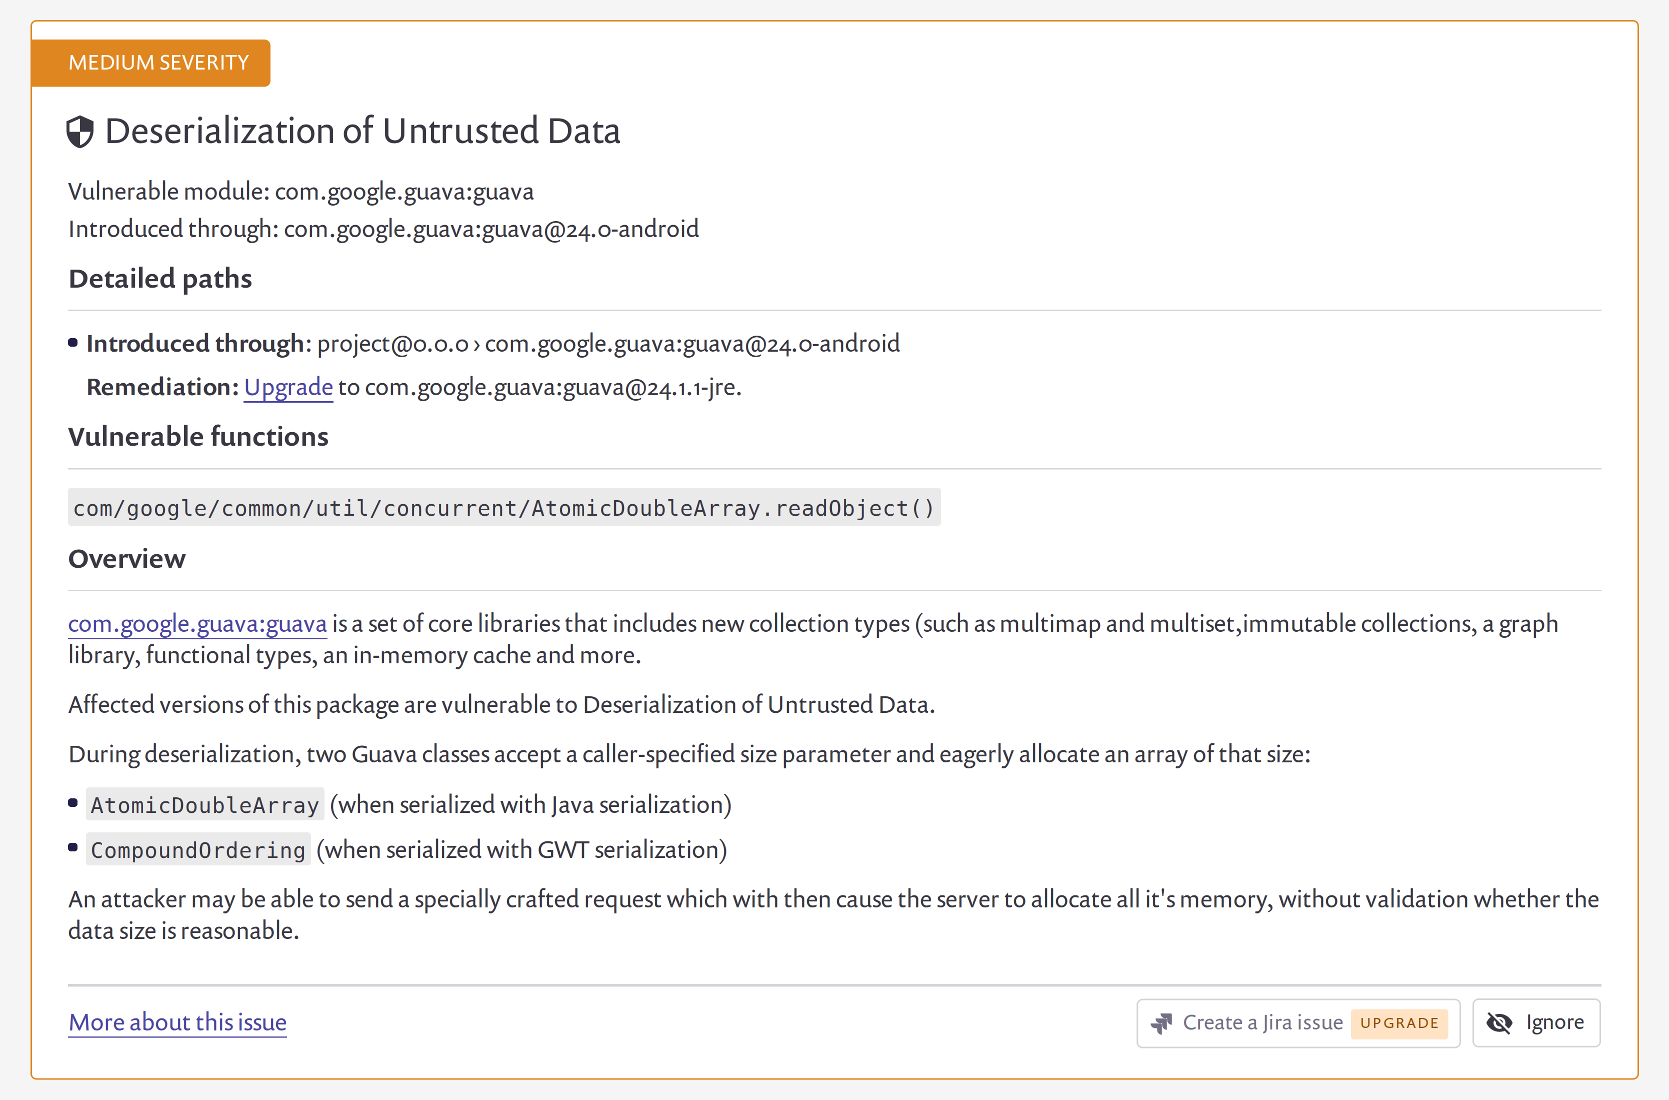
\includegraphics[width=0.9\linewidth]{snyk.png}
    \end{MyMdframed}
\end{figure}

Snyk vulnerabilities relating to deserialisation tend to be raised in large volumes for each \emph{gadget} discovered in
a library.
The system gives no weight to whether the application deserialises user input, does so in an unsafe way which allows any
type to be used, or indeed does any deserialisation at all.
In \emph{My Warwick}'s case, no automatic deserialisation is present at all, and so the is completely unexploitable.
This problem is a consequence of Snyk only analysing dependencies and not performing static analysis on the codebase to
determine if the problem is relevant or not.

At the time of writing, the company has introduced ``runtime monitoring'' to determine if insecure functions are
actually called.
This functionality increases the value of the vulnerability reports, but only supports a limited number of platforms and
requires running an agent alongside the application to collect and send runtime data.

\chapter{Design and Implementation}

This chapter discusses the design decisions made throughout the project and the reasoning behind them.
It additionally covers how the implementation was approached, and the tools and libraries used to produce the prototype.

\section{Design}

The need for our language to be predictable and familiar to developers is clear.
We therefore present an imperative proof-of-concept language, with a C-like syntax.
The aim is that developers, and particularly those that work with JVM technologies, will be able to write critical
sections of code within our language, where regex refinements are available.

This section covers the design of the language's syntax, its type system and the foreign function interface (FFI).

\subsection{Syntax}

As discussed, we had settled on a C-like syntax with some inspiration from other languages such as Go.



\section{Implementation}

\subsection{Frontends}

\subsubsection{Rise4fun}

Within Microsoft Research, the \emph{Research in Software Engineering} (RiSE) group has built a tool known as
\emph{rise4fun}.
This web based tool is an interactive sandbox where allows users interested in programming language research can
experiment with software engineering tooling.
Users can enter code in a syntax-highlighted editor and execute type-checkers and verifiers in their browser.
Results are displayed in real-time.
Showcases exist for projects such as Z3, Dafny and many others.

We natively integrate with Microsoft's Rise4fun platform to showcase our language's features and allow users to
experiment with refinement types.

\begin{figure}[H]
    \begin{MyMdframed}
        \vspace{0.5em}
        
        
        \caption{\label{figure:r4f}Example of a type violation, displayed in the Rise4fun environment.}
        \vspace{0.5em}
        \captionsetup{style=default}
        
        \centering 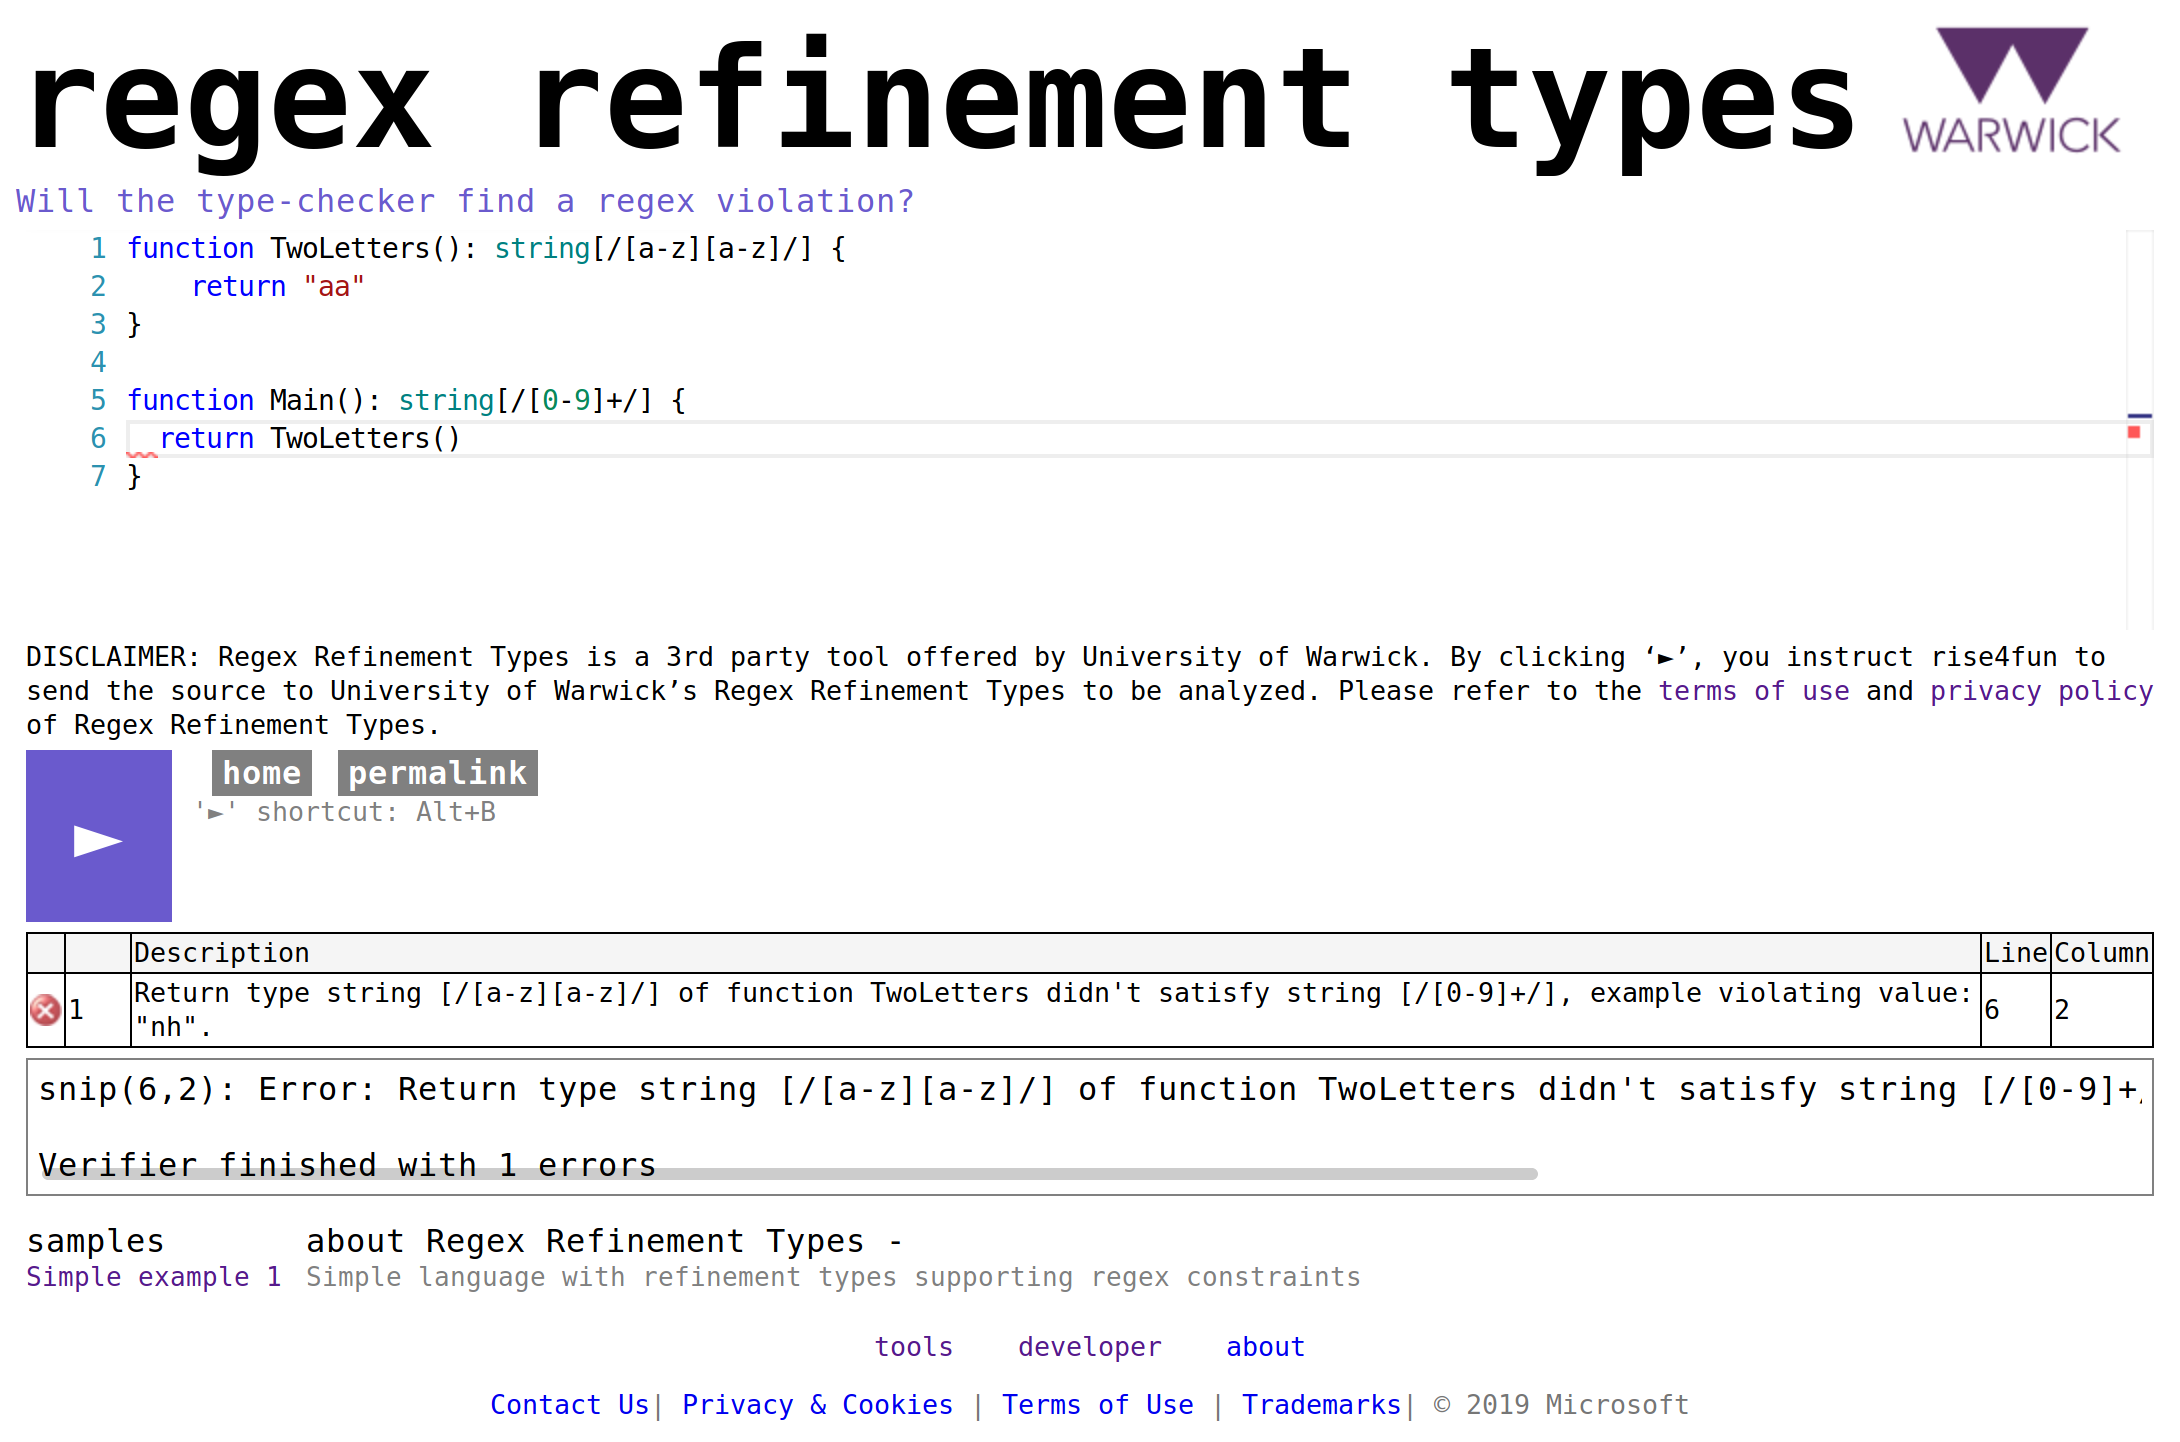
\includegraphics[width=0.9\linewidth]{rise4fun.png}
    \end{MyMdframed}
\end{figure}




\begin{mycodefile}{rrtlex.py:RrtLexer -x}{\label{code:rrt:1}A factorial function written in the RRT language}{RRT}{factorial.rrt}
    \vspace{0.5em}
\end{mycodefile}

\chapter{Testing}

\todobox{Unit testing, manual testing (boundary conditions, adversarial input), integration testing (lexer, parser, interpreter)}

\chapter{Evaluation and Conclusions}

\todobox{This needs to be completed by evaluating not just the performance of the tool against existing static analysis software, but also the scheduling of the project and project management.}

\chapter{Future Work}
\todobox{Flesh this out:\begin{itemize}
        \item Non-regular ``regular expressions'' like we see in PHP, Perl etc
        \item Integration with languages such as C\#--take advantage of Roslyn? Scala/Java could also work by using annotations.
        \item Extend Dafny/Haskell to take advantage of Z3str3?
        \item Or, continue working on the proof of concept language to make it more palatable for serious use
              (more types, generics, .. objects)
\end{itemize}}


\titleformat{\chapter}[display]
{\normalfont \sffamily \Huge  \color{id7-aubergine}}
{}{0pt}{}[]

\bibliographystyle{agsm}
\bibliography{bibliography}

\appendix

\chapter{Project Specification}
\section*{Introduction}

Within information security, entire classes of application vulnerabilities arise due to problematic user input handling \citep{christey2007vulnerability}.
This covers cross-site scripting (XSS), injection (SQL, LDAP, etc), insecure
deserialisation and file inclusion vulnerabilities -- all of which are regularly discovered in major software products.

There are many existing products that aim to detect problems within an application. \citet{sadowski2018lessons} describe the benefits of static analysis tooling deployed within Google which allow checks for common issues to be performed as part of the compilation process. The authors explain one of the main challenges with developer adoption as \emph{trustworthiness} ``users do not trust to results due to, say, false positives`` and highlight the importance of reporting issues early: ``survey participants deemed 74\% of the issues flagged at compile time as real problems, compared to 21\% of those found in checked-in code''.

In the context of application security, tooling can be broadly categorised into the two broad areas of DAST (dynamic application security testing) and SAST (static application security testing) tooling. SAST tooling can analyse a codebase at rest and lends itself to generating much more immediate results that can take the entire codebase into account. DAST tooling allows for assessment from a black-box perspective but is much more limited. Research into the effectiveness of DAST-based scanning tools by \citet{doupe2010johnny} drew the conclusion that commonly available tools of this kind often failed to crawl more complex parts of an application which resulted in decreased coverage from a security perspective.

Existing static analysis tools can provide useful warnings that help prevent introduction of vulnerabilities.
In the .NET ecosystem, tools such as \emph{Roslyn Security Guard} can detect e.g. injection vulnerabilities by tainting
user input and then using information flow analysis -- first described in \cite{denning1977certification} -- to
determine when unsafe input is passed to a dangerous \emph{sink} function \citep{rosylynsecguard}.
Of course, this approach is limited.
All user input is deemed unsafe by virtue of being user input and prior validation (as is commonly performed using
regular expressions) is not taken into account when deciding if an alert needs to be raised or not.
This leads to false positive reports where a program is secure by virtue of already performing validation to prevent a
vulnerability.

The main objective of this project is to explore the use of a type system which uses regular-expression based refinement
types applied to user input.
A refinement type in the context of a type system is a type that is subject to a particular predicate \citep[p.
207]{benjaminpierce2002}.
By considering flow of data that belongs to a refinement type for a particular pattern, it will be possible to make
inferences about vulnerabilities that may be present in a codebase based on declared safe argument types.
Use of refinement types in this way provides for a more informed evaluation of a particular risk than base types alone
and should therefore enable reporting of fewer false positive issues.

\begin{listing}[H]
    \begin{minted}{javascript}
    function LookupName(userId: /[A-Za-z0-9]+/): string {
    var name: string = GetNameByUserId(userId); // safe
    GetNameByUserId("'; DROP TABLE users;"); // type error
    return name;
    }
    
    function GetNameByUserId(query: /[^`"']+/): /[A-Za-z ]+/ { /* database lookup.. */ }
    \end{minted}
    \caption{Example code illustrating a potential syntax. \texttt{userId} and \texttt{query} use the refinement type.}
\end{listing}
\section*{Objectives}



\subsubsection*{Primary Objectives}

\begin{itemize}
    \item Formalise a type system that supports types predicated with a regular expression pattern that elements of the refined type will satisfy (be matched by).
    
    \begin{itemize}
        \item Explore the consequences of typical string operations (e.g. concatenation) and define the type of their return value when applied to elements of the regular expression type.
        
        \item At minimum, this should allow for simple functions to be declared that can safely accept/return a particular regular expression input\footnote{As a simplified example, an \texttt{unsafe\_shell\_exec} function might safely be able to accept any input that matches \texttt{\textasciicircum{}[\textasciicircum{}\textasciigrave{}]\textdollar{}}}.
        
        \item Evaluate the rate of false positives when compared to existing static analysis 
    \end{itemize}
    
    \item Implement such a type system that can guarantee type safety, built against a simplified proof-of-concept language.
    \begin{itemize}
        \item Test the implementation against a variety of test cases. The testing strategy should make use of automated unit tests, and manual system testing considering both general expected input as well as any relevant ``edge-cases'' that need to be handled.
    \end{itemize}
\end{itemize}

\subsubsection*{Additional Objectives}

\begin{itemize}
    \item Apply the theory explored in the primary phase of the project to produce a type analysis tool which works against type annotations applied to a commonly-used language such as C\# or Scala. This tooling could be integrated into an IDE or CI pipeline.
\end{itemize}

\textit{}\infobox{Primary objectives are expected to be completed during the lifetime of the project. Additional objectives are identified as potential goals to pursue beyond the original scope of the project, if time permits.}

\section*{Schedule}

\arrayrulecolor{white}
\def\arraystretch{1.5}
\begin{table}[H]
    
    \centering
    \rowcolors{1}{id7-sky-blue-tint}{lightgrey}
    \begin{tabular}[t]{|p{5.5cm}|p{10cm}|}
        \hline
        \rowcolor{id7-sky-blue}
        {\color[HTML]{FFFFFF} \sffamily \textbf{Time Window}} & {\color[HTML]{FFFFFF} \sffamily \textbf{Work}} \\ \hline
        October \nth{1} -- October \nth{14} & Specification completion, research into prior related works. Study of elementary programming language and type system theory (e.g. simply typed $\lambda$-calculus, SLam). \\ \hline
        October \nth{15} -- October \nth{28} & \parbox[t]{10cm}{Begin writing background for report, work on formalisation of regular expression refinement type.\\\textcolor{id7-ruby-red}{\textbf{Deadline}: CS353 presentation, \nth{24} October}}\vspace{0.4em} \\ \hline
        October \nth{29} -- November \nth{11} & Explore and document properties of type system. Begin implementation of ideas to produce a concrete proof-of-concept. \\ \hline
        November \nth{12} -- November \nth{25} & Completion of progress report, continued implementation work. \\ \hline
        November \nth{26} -- December \nth{9} & \parbox[t]{10cm}{Testing of implemented proof-of-concept.\\\textcolor{id7-ruby-red}{\textbf{Deadline}: CS915 coursework, \nth{26} November}}\vspace{0.4em} \\ \hline
        December \nth{10} -- January \nth{6} & Slack time (to use if behind schedule, else to make a start on year scheduled in 2019). \\ \hline
        January \nth{7} -- January \nth{20} & \parbox[t]{10cm}{Finalise testing of implementation, write-up test cases.\\\textcolor{id7-ruby-red}{\textbf{Deadline}: CS324 coursework}}\vspace{0.4em} \\ \hline
        January \nth{21} -- February \nth{3} & Evaluate false positive rates against existing systems based exclusively on taint tracking. \\ \hline
        February \nth{4} -- February \nth{17} & Report work, project presentation preparation \\ \hline
        February \nth{18} -- March \nth{3} & Project presentation preparation, report work \\ \hline
        March \nth{4} -- March \nth{17} & Project presentation delivery, report finalisation. \\ \hline
    \end{tabular}
    \caption{Projected work by time period. Deadlines for other modules included where known.}
    \label{schedule}
\end{table}

Table \ref{schedule} provides a breakdown of the project time into periods for each fortnight, along with the expected work to be completed. A meeting will be scheduled for each week to discuss progress and any road-blocks that arise with the project supervisor

\section*{Methodology}

\subsection*{Software Engineering}

This project includes an element of software engineering. Namely, the design and implementation of a proof of concept language which supports a type system incorporating regular expression refinement types.

This implementation work will be carried out in an Agile fashion to fit in with the short timescales inherent to the project and allow for greater flexibility. Time periods in the schedule which involve development work will be treated as a number of week-long development sprints with priorities formalised prior to the commencement of each period. Progress will be reviewed in weekly supervision meetings.

Testing will be automated via the use of unit testing to ensure that specific components function according to their specification in isolation. Where appropriate, integration and system testing can be used to test the solution as a whole (for example, an entire program as a test case would fit into this part of the testing process).

\subsection*{Evaluation}

Towards the end of the implementation phase, the false positive rate of the proof of concept tool should be compared with that of existing static analysis tooling based on taint tracking alone.

Logically equivalent test cases should be built for each tool under evaluation in the necessary programming language. Both safe and unsafe function invocations should be included in each test case for completeness.

\section*{Resources and risks}


The project is reliant on a number of resources. Use of these resources is subject to the risks outlined in table \ref{rr}. These risks should be evaluated and managed to minimise any potential impact on the project.

\arrayrulecolor{white}
\def\arraystretch{1.5}
\begin{table}[H]
    
    \centering
    \rowcolors{1}{id7-sky-blue-tint}{lightgrey}
    \begin{tabular}[t]{|p{5.5cm}|p{4cm}|p{7cm}|}
        \hline
        \rowcolor{id7-sky-blue}
        {\color[HTML]{FFFFFF} \sffamily \textbf{Resource}} & {\color[HTML]{FFFFFF} \sffamily \textbf{Applicable risk(s)}} &
        {\color[HTML]{FFFFFF} \sffamily \textbf{Impact}} \\ \hline
        \parbox[t]{5cm}{\textbf{VCS hosting: GitHub}\\Storing and tracking code and report changes\\} & Loss of availability due to outage & Minimal, \emph{git} is decentralised so copy of files always available locally and at off-site backup \\ \hline
        \parbox[t]{5cm}{\textbf{Report authoring: \LaTeX}\\Writing and compiling the report, tracking bibliography} & Obsolescence & Unlikely, TeX tooling has been used for decades. Even if particular packages ceased working, the bulk of the content would still be accessible as plain text. \\ \hline
        \parbox[t]{5cm}{\textbf{C\# analysis: Roslyn libary}\\Fulfilling the additional objective by analysing C\# code} & Loss of availability due to license change & Minimal. Even if Roslyn's OSS status changes, there is no requirement to integrate with C\#, other languages would illustrate the potential just as well. This would also not impact a primary project objective. \\ \hline
        \parbox[t]{5cm}{\textbf{Self}\\Project work} & Illness, coursework deadlines & Minimised by scheduled slack time and identification of applicable coursework deadlines. \\ \hline
    \end{tabular}
    \caption{Resources and associated risks. \label{rr}}
\end{table}


\section*{Legal, social, ethical and professional issues}

As a project with some security motivation, it is possible that legal, social, ethical and professional issues will arise. In particular, evaluation of existing static analysis tooling must be performed with care to ensure that use of any particular external test cases is permitted by the \emph{Copyright, Designs and Patents Act 1988} within the UK.

Additionally, in order to comply with the \emph{Computer Misuse Act 1988}, any static analysis of external code should only be conducted with permission.  Discovered issues should be disclosed responsibly.

\end{document}
